\chapter{embed-tree.h Documentation}
\ifsingle
\maketitle
\fi
\chaptermeta[draft][2025-06-09]

\section{Introduction}
This header file provides restriction, prolongation, and refinement operations under a tree grid for values used in \textbf{embed.h}. The content is divided into two parts: the refinement of cut-cell values, i.e., \para{cs} and \para{fs}, and the restriction/prolongation of values on cut-cells and cut-faces.

\section{Refinement of Embed-Associated Values}
\subsection{\func{embed\_fraction\_refine}}
The \func{embed\_fraction\_refine} function calculates the volume fraction contained by each child cell.

\subsubsection{Worth Mentioning Details}
\begin{figure}[ht]
    \centering
    \begin{subfigure}[b]{0.45\textwidth}
        \centering
        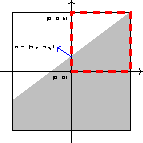
\includegraphics[height=6cm]{./image/embed-tree-h/fraction_refine2D1.pdf}
        \subcaption{}
        \label{fig:embed-tree-2Drefine1}
    \end{subfigure}
    \begin{subfigure}[b]{0.45\textwidth}
        \centering
        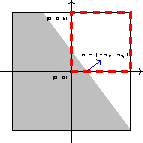
\includegraphics[height=6cm]{./image/embed-tree-h/fraction_refine2D2.pdf}
        \subcaption{}
        \label{fig:embed-tree-2Drefine2}
    \end{subfigure}
    \caption{Refinement of embed fraction \para{cs}. By switching the component of the normal direction $\mathbf{n}$, the program rotates the interface, thereby iterating the volume fraction of each subcell.}
    \label{fig:embed-tree-2Drefine}
\end{figure}
For cells containing an interface, given the function \func{rectangle\_fraction} from \textbf{geometry.h} and interface information $\mathbf{n}$, $\alpha$, the volume fraction inside each child cell can be obtained. As shown in figure \ref{fig:embed-tree-2Drefine1}, under a 2D condition, the area inside the child cell highlighted by a red dashed line is calculated.

Instead of switching the computational domain (i.e., the red dashed cell), the program iterates between cells by switching the sign of the normal direction, as indicated in figure \ref{fig:embed-tree-2Drefine2}.

\subsubsection{Parameters}
\begin{center}
  \begin{tabular}{|c|c|c|c|c|}
    \hline
    Name & Data type & Status & Option & Representation (before/after)\\[0.5ex]
    \hline\hline
    \para{point} & Point & unchanged & compulsory & position index\\
    \hline
    \para{cs} & scalar & unchanged & compulsory & volume fraction $cs$\\
    \hline
  \end{tabular}
\end{center}

\begin{codesection}{subsubsection}{Program Workflow}
\codecomment{
  \textbf{Starting Point}\\
  \textbf{Input}: \para{cs} = $cs$, the volume fraction, \para{cc} = $cs[]$.\\
  \textbf{Non-Interfacial Cell}: For full or empty cells, the volume fraction of child cells is directly inherited from the parent cell.
}
\begin{minted}{cpp}
static void embed_fraction_refine (Point point, scalar cs)
{
  double cc = cs[];
  if (cc <= 0. || cc >= 1.) {
    foreach_child()
      cs[] = cc;
  }
\end{minted}
\codearrow
\codecomment{
  \textbf{Refinement of Volume Fraction on Interfacial Cell}\\
  \textbf{Interface Information}: \para{n} = $\mathbf{n}$, \para{alpha} = $\alpha$.\\
  \textbf{Volume Fraction Refinement}: After iterating each child cell using the macro \texttt{foreach\_child}, the computational domain is confined with coordinates \para{a} and \para{b} (the red square in figure \ref{fig:embed-tree-2Drefine}). An additional normal direction \para{nc} is defined to switch between child cells (see `vof.h' documentation for the definition of index \para{child.x}). The volume fraction for each child cell is then obtained.
}
\begin{minted}{cpp}
    coord n = facet_normal (point, cs, fs);
    double alpha = plane_alpha (cc, n);
      
    foreach_child() {
      static const coord a = {0.,0.,0.}, b = {.5,.5,.5};
      coord nc;
      foreach_dimension()
        nc.x = child.x*n.x;
      cs[] = rectangle_fraction (nc, alpha, a, b);
    }
  }
}
\end{minted}
\end{codesection}

\subsection{\func{embed\_face\_fraction\_refine}}
Given the face vector \para{fs} on mesh level $N$, the function \func{embed\_face\_fraction\_refine} returns \para{fs} on the finer mesh level $N+1$. The computation of face fractions is achieved by first calculating the fractions of `inner' faces, followed by `boundary' faces, under both 2D and 3D conditions. For clarity, the implementation for 2D cases is introduced first, followed by 3D cases. However, the program is organized based on computations for `inner' or `boundary' faces.

Note that the function is duplicated by the macro \texttt{foreach\_dimension}, and each instance is responsible for face fraction computation in one direction. The following explanation uses the $x$-direction as an example.

Moreover, for a cut-cell ($\para{cs} \in (0,1)$), the interface is defined by:
\begin{equation}\label{equ:embed-tree-interface}
    \mathbf{n} \cdot \mathbf{x} = \alpha
\end{equation}
where $\mathbf{n}$ is the normal direction of the interface, $\mathbf{x}$ represents the coordinates of any point on the interface, and $\alpha$ is a constant. This equation is critical for identifying different conditions in the following sections.

\subsubsection{2D Condition}
First, consider the fine faces contained inside the cell, as shown by $A$ and $B$ in figure \ref{fig:embed-tree-2Dinner}.

\begin{figure}[ht]
    \centering
    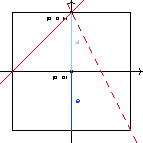
\includegraphics[height=6cm]{./image/embed-tree-h/fs_2D.pdf}
    \caption{Sketch of inner fine faces $A$, $B$. The two red lines represent example threshold values for the interfaces.}
    \label{fig:embed-tree-2Dinner}
\end{figure}

The initial step in computing face fractions is to determine whether the interface intersects the inner fine faces. Given $\alpha = \alpha_1$ and $\mathbf{n} = (n_x, n_y)$ for the interface, and a coordinate system with $(0,0)$ at the cell’s center, the lower and upper boundaries are lines passing through $(0,0.5)$ and $(0,-0.5)$, respectively. According to equation \ref{equ:embed-tree-interface}, if:
\begin{equation}\label{equ:embed-tree-judge}
    |2\alpha_1| < |n_y|
\end{equation}
the interface intersects the inner fine faces; otherwise, both face fractions are $0$ or $1$, depending on the interface’s direction. If equation \ref{equ:embed-tree-judge} holds, the intersection point $(0, y_i)$ between the interface and the $y$-axis is $y_i = \frac{\alpha}{n_y}$. The face fractions for faces $A$ and $B$ can then be computed accordingly.

\begin{figure}[ht]
    \centering
    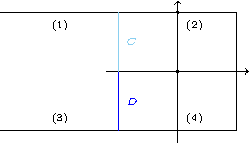
\includegraphics[height=6cm]{./image/embed-tree-h/fs_2D2.pdf}
    \caption{Sketch of boundary fine faces $C$, $D$. The numerical labels mark the corresponding transverse faces.}
    \label{fig:embed-tree-2Dboundary}
\end{figure}

For boundary fine faces, a similar process is followed: first, identify the intersection point (if it exists), then compute the fine face fraction. Unlike the inner faces, boundary face fractions can be accessed directly without checking equation \ref{equ:embed-tree-judge}. The interface’s orientation is determined by examining the corresponding transverse faces, as shown by labels (1–4) in figure \ref{fig:embed-tree-2Dboundary}. Combined with the face fraction on the original face, the fine face fraction is obtained.

\subsubsection{3D Condition}
\begin{figure}[ht]
    \centering
    \begin{subfigure}[b]{0.45\textwidth}
        \centering
        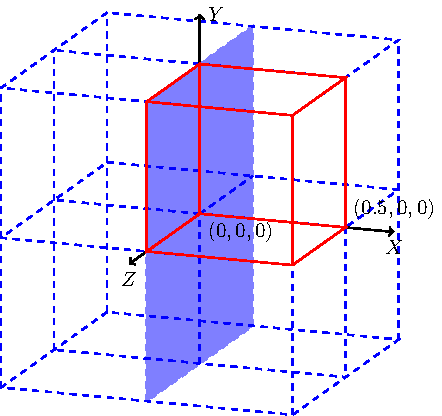
\includegraphics[height=6cm]{./image/embed-tree-h/fs_3D3.pdf}
        \subcaption{}
        \label{fig:embed-tree-3Dinner}
    \end{subfigure}
    \begin{subfigure}[b]{0.45\textwidth}
        \centering
        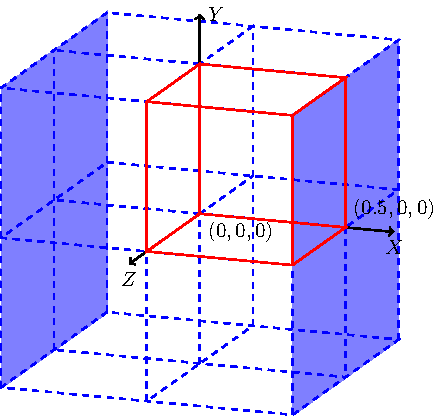
\includegraphics[height=6cm]{./image/embed-tree-h/fs_3D4.pdf}
        \subcaption{}
        \label{fig:embed-tree-3Dboundary}
    \end{subfigure}
    \caption{Inner fine face (a) and boundary fine face (b) under 3D conditions. The red contour highlights the cell where projection takes place.}
    \label{fig:embed-tree-3Dface}
\end{figure}

\begin{figure}[ht]
    \centering
    \begin{subfigure}[b]{0.45\textwidth}
        \centering
        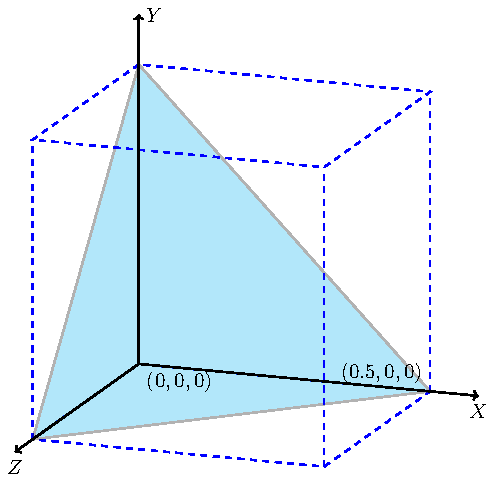
\includegraphics[height=6cm]{./image/embed-tree-h/fs_3D1.pdf}
        \subcaption{}
        \label{fig:embed-tree-3Dinner1}
    \end{subfigure}
    \begin{subfigure}[b]{0.45\textwidth}
        \centering
        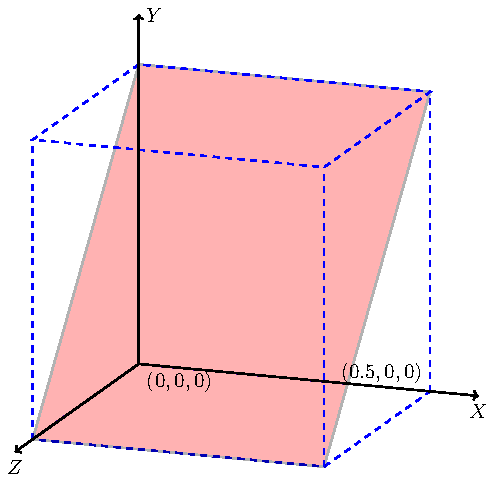
\includegraphics[height=6cm]{./image/embed-tree-h/fs_3D2.pdf}
        \subcaption{}
        \label{fig:embed-tree-3Dinner2}
    \end{subfigure}
    \begin{subfigure}[b]{0.45\textwidth}
        \centering
        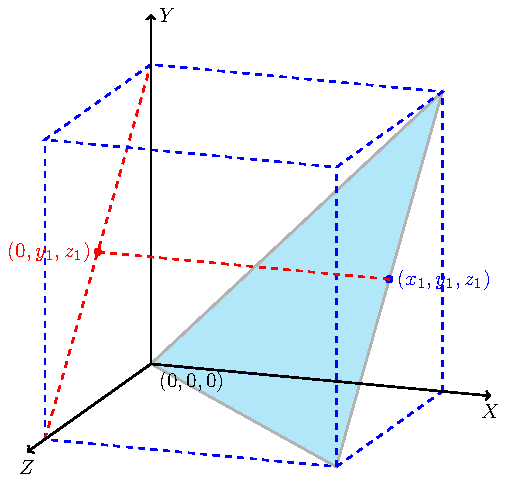
\includegraphics[height=6cm]{./image/embed-tree-h/fs_3D5.pdf}
        \subcaption{}
        \label{fig:embed-tree-3Dinner3}
    \end{subfigure}
    \caption{Zoom-in view of the highlighted cell in figure \ref{fig:embed-tree-3Dface}. (a) The original interface, (b) the projected interface for the inner face in figure \ref{fig:embed-tree-3Dinner}, and (c) the original interface for the boundary fine face in figure \ref{fig:embed-tree-3Dboundary}.}
    \label{fig:embed-tree-3DinnerZoom}
\end{figure}

The fine face fractions for both inner and boundary faces are computed directly using 2D projections from a 3D interface.

For the inner face, as shown in figure \ref{fig:embed-tree-3Dinner}, the fine face fraction is computed from a 2D projection in the red-contoured cell. Iteration among the four subcells is achieved by rotating the entire interface, as described in section (unfinished). Given $\mathbf{n} = (n_x, n_y, n_z)$ and $\alpha = \alpha_1$ for the example interface in figure \ref{fig:embed-tree-3Dinner1}, the face fraction on the inner fine face is obtained by calculating the volume fraction of the reconstructed interface shown in figure \ref{fig:embed-tree-3Dinner2}. Since volume calculations are supported by tools in \textbf{geometry.h}, the problem reduces to reconstructing the interface and determining its $\mathbf{n}$ and $\alpha$.

The reconstructed interface is perpendicular to the projection plane and intersects the same line as the original interface on the projection plane, with $\mathbf{n} = (0, n_y, n_z)$ and $\alpha = \alpha_1$.

Similarly, the fine face fraction on the boundary face is computed by projection onto the boundary plane. As shown in figure \ref{fig:embed-tree-3Dinner3}, the reconstructed plane must pass through the intersection line on the boundary face (blue line) and the red dashed line. Given an arbitrary point set $(0.5, y_1, z_1)$ and $(0, y_1, z_1)$, the $\alpha = \alpha_2$ of the reconstructed interface satisfies:
\begin{align}
    0.5 n_x + y_1 n_y + z_1 n_z &= \alpha_1\\
    y_1 n_y + z_1 n_z &= \alpha_2\\
    \alpha_2 &= \alpha_1 - 0.5 n_x \label{equ:embed-tree-alphabf}
\end{align}
With the normal direction $(0, n_y, n_z)$, the face fraction can be calculated.

\subsubsection{Worth Mentioning Details}
\begin{figure}[ht]
    \centering
    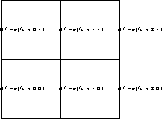
\includegraphics[height=6cm]{./image/embed-tree-h/fine.pdf}
    \caption{Index for \func{fine}.}
    \label{fig:embed-tree-finefunc}
\end{figure}

In addition to geometric formulas, the function \func{fine} is called multiple times to access data on the finer mesh. The index for the face vector of a subcell is shown in figure \ref{fig:embed-tree-finefunc}, which can be directly extended to 3D conditions.

\subsubsection{Parameters}
\begin{center}
  \begin{tabular}{|c|c|c|c|c|}
    \hline
    Name & Data type & Status & Option & Representation (before/after)\\[0.5ex]
    \hline\hline
    \para{point} & Point & unchanged & compulsory & position index\\
    \hline
    \para{s} & scalar & unchanged & compulsory & volume fraction $cs$\\
    \hline
  \end{tabular}
\end{center}

\begin{codesection}{subsubsection}{Program Workflow}
\codecomment{
  \textbf{Starting Point}\\
  \textbf{Input}: \para{s} = $cs$, face vector attributed with volume fraction, i.e., \para{fs} = $s.v$.\\
  \textbf{Full \& Empty Cell}: For full and empty cells, the face fraction is directly assigned the parent value. For boundary fine face fractions, a check ensures consistency with neighboring cells.
}
\begin{minted}{cpp}
foreach_dimension()
static void embed_face_fraction_refine_x (Point point, scalar s)
{
  vector fs = s.v;
  if (cs[] <= 0. || cs >= 1.) {
    for (int j = 0; j <= 1; j++)
      for (int k = 0; k <= 1; k++)
        fine(fs.x,1,j,k) = cs[];
    for (int i = 0; i <= 1; i++)
      if (!is_refined(neighbor(2*i-1)) && neighbor(2*i-1).neighbors &&
          (is_local(cell) || is_local(neighbor(2*i-1))))
        for (int j = 0; j <= 1; j++)
          for (int k = 0; k <= 1; k++)
            fine(fs.x,2*i,j,k) = fs.x[i];
  }
\end{minted}
\codearrow
\codecomment{
  \textbf{Computation of Inner Fine Face Fraction}\\
  \textbf{Interfacial Information}: Since the current cell contains an interface, obtain \para{n} = $\mathbf{n}$, \para{alpha} = $\alpha$.\\
  \textbf{2D Condition}: For interfaces satisfying equation \ref{equ:embed-tree-judge}, which cut through the inner face, compute the fine face fraction using the intersection $y_i = \frac{\alpha}{n_y}$. Otherwise, the fine face fraction is full or empty.\\
  \textbf{3D Condition}: As discussed, compute the fine face fraction from the volume fraction of the reconstructed interface with $\mathbf{n}_{re} = (0, n_y, n_z)$, $\alpha_{re} = \alpha$. Iteration between subcells is implemented by rotating the original cell.
}
\begin{minted}{cpp}
  else {
    coord n = facet_normal (point, cs, fs);
    double alpha = plane_alpha (cs[], n);
#if dimension == 2
    if (2.*fabs(alpha) < fabs(n.y)) {
      double yc = alpha/n.y;
      int i = yc > 0.;
      fine(fs.x,1,1 - i) = n.y < 0. ? 1. - i : i;
      fine(fs.x,1,i) = n.y < 0. ? i - 2.*yc : 1. - i + 2.*yc;
    }
    else
      fine(fs.x,1,0) = fine(fs.x,1,1) = alpha > 0.;
#else // dimension == 3
    for (int j = 0; j <= 1; j++)
      for (int k = 0; k <= 1; k++)
        if (!fine(cs,0,j,k) || !fine(cs,1,j,k))
          fine(fs.x,1,j,k) = 0.;
        else {
          static const coord a = {0.,0.,0.}, b = {.5,.5,.5};
          coord nc;
          nc.x = 0., nc.y = (2.*j - 1.)*n.y, nc.z = (2.*k - 1.)*n.z;
          fine(fs.x,1,j,k) = rectangle_fraction (nc, alpha, a, b);
        }
#endif // dimension == 3
\end{minted}
\codearrow
\codecomment{
  \textbf{Computation of Boundary Fine Face Fraction}\\
  \textbf{Full/Empty Cell Detection}: For full/empty cells, assign fine face fractions as $1$/$0$.\\
  \textbf{2D Condition}: Follow the procedure described to compute boundary fine face fractions.\\
  \textbf{3D Condition}: Compute boundary fine face fractions using equation \ref{equ:embed-tree-alphabf} for $\alpha_{re}$.
}
\begin{minted}{cpp}
    for (int i = 0; i <= 1; i++)
      if (neighbor(2*i-1).neighbors &&
          (is_local(cell) || is_local(neighbor(2*i-1)))) {
        if (!is_refined(neighbor(2*i-1))) {
          if (fs.x[i] <= 0. || fs.x[i] >= 1.)
            for (int j = 0; j <= 1; j++)
              for (int k = 0; k <= 1; k++)
                fine(fs.x,2*i,j,k) = fs.x[i];
          else {
#if dimension == 2
            double a = fs.y[0,1] <= 0. || fs.y[2*i-1,1] <= 0. ||
              fs.y[] >= 1. || fs.y[2*i-1] >= 1.;
            if ((2.*a - 1)*(fs.x[i] - 0.5) > 0.) {
              fine(fs.x,2*i,0) = a;
              fine(fs.x,2*i,1) = 2.*fs.x[i] - a;
            }
            else {
              fine(fs.x,2*i,0) = 2.*fs.x[i] + a - 1.;
              fine(fs.x,2*i,1) = 1. - a;
            }
#else // dimension == 3
            for (int j = 0; j <= 1; j++)
              for (int k = 0; k <= 1; k++) {
                static const coord a = {0.,0.,0.}, b = {.5,.5,.5};
                coord nc;
                nc.x = 0., nc.y = (2.*j - 1.)*n.y, nc.z = (2.*k - 1.)*n.z;
                fine(fs.x,2*i,j,k) =
                  rectangle_fraction (nc, alpha - n.x*(2.*i - 1.)/2., a, b);
              }
#endif // dimension == 3
          }
        }
\end{minted}
\codearrow
\codecomment{
  \textbf{Confirmation of Empty Cell}\\
  Ensure the face fraction is $0$ for empty cells.
}
\begin{minted}{cpp}
        for (int j = 0; j <= 1; j++)
        #if dimension > 2
          for (int k = 0; k <= 1; k++)
        #endif
            if (fine(fs.x,2*i,j,k) && !fine(cs,i,j,k))
              fine(fs.x,2*i,j,k) = 0.;
      }
  }
}
\end{minted}
\end{codesection}
\printbibliography
